\icode{E-MI-SI-L3-261108-003}
如图所示，光滑半圆形轨道固定在竖直平面内，\(MN\)为水平直径，一轻质小环\(A\)套在轨道上，轻绳一端固定在\(M\)点，另一端穿过小环系一质量为\(m\)的小球恰好静止在图示位置，不计所有摩擦，重力加速度大小为\(g\)。下列说法正确的是\paren[]
	
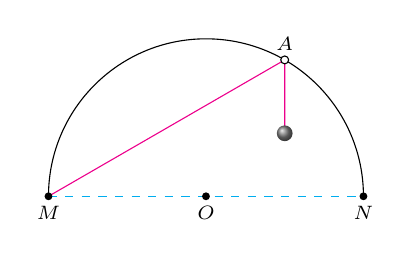
\begin{tikzpicture}[font=\scriptsize]
	\draw (-2,0) arc(180:0:2);
	\draw[dashed,cyan] (-2,0)node[below,black]{\(M\)}--(2,0)node[below,black]{\(N\)};
	\draw[magenta] (-2,0)--(60:2)--(1,.8);
	\shade[ball color=gray] (1,.8) circle(.1);
	\draw[fill=white] (60:2)node[above]{\(A\)} circle(.05);
	\fill (-2,0) circle(.05) (2,0) circle(.05) (0,0)node[below]{\(O\)} circle(.05);
\end{tikzpicture}
\begin{choices}
	\item 轻绳对\(M\)点拉力的大小为\(\dfrac{\sqrt{3}}{2}mg\)
	\item 轻绳对\(M\)点拉力的大小为\(2mg\)
	\item 轻绳对小环\(A\)作用力的大小为\(\sqrt{3}mg\)
	\item 轻绳对小环\(A\)作用力的大小为\(2mg\)
\end{choices}
\begin{answer}
	C\qquad 提示：
\end{answer}